\section{Introduction}

\subsection{Background}
    The most popular replacement heart valves continue to be bioprosthetic heart valves (BHV) fabricated from xenograft biomaterials, for both established surgical and more novel percutaneous valve designs \cite{schoen_evolving_2008,schoen_new_2006,schoen_cardiac_2005,schoen_calcification_2005,schoen_pathology_2001}. While these devices have provided great benefits for many patients, device failure continues to be the result of leaflet structural deterioration mediated by fatigue and/or tissue mineralization \cite{vesely_tissue_2001,sacks_collagen_2002}. As a result, the lifespan of BHVs remains limited to 10–15 years and the mechanisms that underlie such failures remain poorly understood. Thus, improved durability remains an important clinical goal and represents a unique cardiovascular engineering challenge resulting from the extreme valvular mechanical demands. Yet, current BHV assessments rely exclusively on device-level evaluations, which are confounded by simultaneous and highly coupled biomaterial mechanical fatigue, valve design, hemodynamics, and calcification. Thus, despite decades of clinical BHV usage and growing popularity, there exists no acceptable method for simulating BHV durability in any design context. While efforts to mitigate tissue mineralization have progressed well, efforts to minimize structural degradation remain limited. For example, in vitro accelerated wear tests (AWT) are used only for the most basic device-level durability evaluations. Yet no systematic attempt has been made to glean important durability information from these required tests to inform mechanisms and means to simulate BHV durability. There is thus a profound need for the development of novel simulation technologies for the prediction of the changes in the properties of BHVs to long-term cyclic loading.
    
    
\subsection{Mechanisms of BHV failure}

    The causes of BHV failure can be divided into two broad categories, mineralization, and structural damage, with both processes occurring in parallel or independently \cite{sacks_collagen_2002}. Mineralization is the accumulation of mineral deposits, mainly calcium phosphate, within the BHV leaflets \cite{schoen_calcification_2005}. This disrupts the underlying microstructure preventing the proper mechanical function of BHVs, increasing the likelihood of tearing, and reducing flexibility (preventing normal opening and closing motions, and induce valve stenosis). The causes of calcification and associated anti-calcification treatments are extensively studied in literature \cite{park_novel_1997, isenburg_tannic_2005, vyavahare_prevention_1997}. On the other hand, structural damage includes the collagen fiber damage and breakdown of the non-fibrous part of the extracellular matrix (ECM), \emph{which we will refer to as simply the matrix}. Fourier transform infrared spectroscopy(FTIR) results have shown changes in the collagen fiber molecular structure after 50 million cycles \cite{sun_response_2004}, which suggests that some collagen fiber damage has occurred during this period. However, its effect on the mechanical response of BHVs was not detectable. Nevertheless, it is important to maintain the structural integrity of the BHV, as this will help to improve BHV durability.
    

\subsection{Constitutive model of BHV biomaterial under permanent set}

    In previous chapters, we developed a constitutive model for the underlying mechanical properties of collagenous soft tissues used to fabricate BHVs (Chapter 2, 3) as well as the extensions for the evolution of the material properties in response to permanent set (Chapter 4). The constitutive model utilizes the mechanisms at the meso-scale (i.e. at the level of the fiber, 10-100 $\mu$m in length scale), takes into account the layered structure of these tissue and the contributions from the distinct collagen and elastin fiber networks within each tissue layer to predict the mechanical response at the tissue scale. This approach was further extended for the effect of crosslinking on the fiber matrix interactions to simulate exogenously crosslinked materials. Requisite collagen and elastin fibrous structural information can be obtained using microscopy and conventional histology, and the approach was validated using a novel fibril-level (0.1 to 1 $\mu$m) approach to compare the predicted collagen fiber/fibril mechanical behavior with extant MV small angle X-ray scattering data. 
    
    
    Permanent set is the significant changes in the geometry of BHVs observed in experimental studies \cite{smith_fatigue_1999}\cite{smith_high_1997} with in vivo operation. This can lead to stress concentrations that can have a significant impact on structural damage. Structural damage was not detected in the time frame when permanent set is the most dominant. We hypothesize that the scission-healing reaction of glutaraldehyde is the underlying mechanism responsible for permanent set in exogenously crosslinked soft tissues. The continuous scission-healing process of glutaraldehyde allows a portion of the exogenously crosslinked matrix, which is considered to be the non-fibrous part of the extracellular matrix, to be re-crosslinked in the loaded state. We model the permanent set effect in chapter 4 by assuming that the exogenously crosslinked matrix undergoes changes in reference configurations over time. The changes in the collagen fiber architecture due to dimensional changes allow us to predict subsequent changes in mechanical response. A key finding we have is that the collagen fiber architecture has a limiting effect on the maximum changes in geometry that the permanent set effect can induce. This is due to the recruitment of collagen fibers as the changes in geometry due to permanent set increase. This means we can potentially optimize the BHV geometry based on the predicted the final BHV geometry after permanent set has largely ceased. 
    

\subsection{Numerical simulation framework}

    However, numerical simulations using our constitutive model for permanent set is quite costly. Due to the incorporation of the quadruple integral to calculate fiber interactions, the resulting computational cost is five magnitudes higher than conventional phenomenological approaches. It is for this reason that we developed an effective constitutive model for planar soft tissues and a parameter estimation approach for rapidly determining the model parameters from the micro-model. This approach takes advantage of the computationally efficient forms of phenomenological models and the mechanisms and predictive capabilities of micro-models (meso-scale, multi-scale, or other complex constitutive models) (Fig. \ref{fig:simulationframework}A). For each iteration of the simulation, whether forward, inverse, or time-evolving, the effective constitutive model is first fit to the micro-model(s) to determine the model parameters, then it is used to perform the actual numerical simulation. Subsequent updates to the evolving material properties, geometry, and boundary conditions are then performed (Fig. \ref{fig:simulationframework}B). This approach can greatly improve the computational efficiency of numerical simulations and make it possible for a finite element implementation of the permanent set simulation (Chapter 4). In this chapter, we develop and numerical simulation framework for the time evolving properties of BHVs in response to permanent set, and attempt to predict the geometric and structural change that occurs with long-term cyclic loading. 
    
%%%%%%%%%%%%%%%%%%%%%%%%%%%%%%%%%%%%%%%%%%%%%%%%%%%%%%%%%%%%
%-------------------	begin FIGURE 	-------------------%
\begin{figure}
\centering
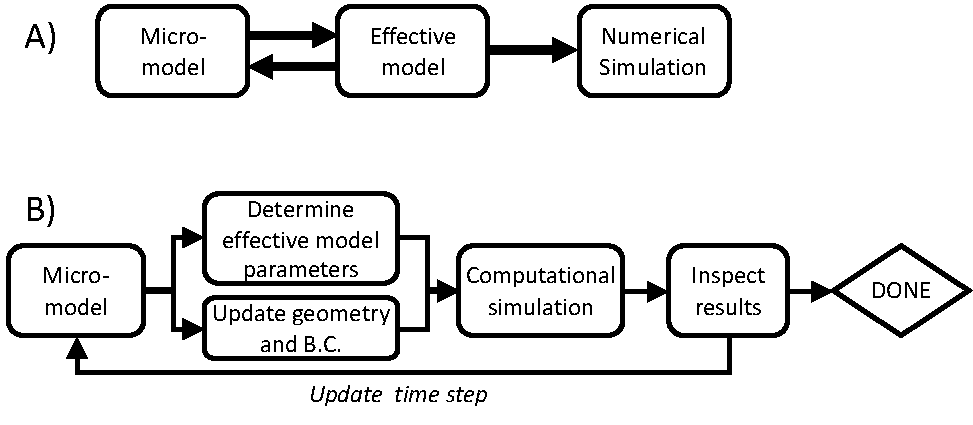
\includegraphics[width=\textwidth]{Images/chapter5/simulationframework}
\caption{Proposed frame work for using an effective constitutive model to improve the efficiency of using complex meso- or multi-scale models (micro\Hyphdash models) in numerical simulations. Here, A) effective constitutive models act as an intermediate step between micro-models and numerical simulations, where micro-models inform the changes to the effective constitutive model while the effective constitutive model for the simulation. B) An example of how this may be implemented for time\Hyphdash evolving is shown.}
\label{c6:fig:simulationframework}
\end{figure}
%-------------------	 end FIGURE 	-------------------%
%%%%%%%%%%%%%%%%%%%%%%%%%%%%%%%%%%%%%%%%%%%%%%%%%%%%%%%%%%%%
    
    